\documentclass{iopconfser}

\usepackage{float}
\usepackage{graphicx}
\usepackage{subcaption}
\usepackage[automake]{glossaries-extra}
\usepackage{ragged2e}

% \makeglossaries

\setabbreviationstyle[acronym]{long-postshort-user}
\glssetcategoryattribute{acronym}{nohyperfirst}{true}
\setabbreviationstyle{short-nolong}
\makeglossaries

% --------------------
% ---- Glossaries ----
% --------------------
\newglossaryentry{asyncio}{name=Asyncio, description={A Python library for asynchronous code.}}
\newglossaryentry{stim}{name=STIM300, description={A MEMS-based \gls{imu}}}
\newglossaryentry{f9p}{name=F9P, description={A Global Navigation Satellite System (GNSS) receiver manufactured by u-blox.}}

% --------------------
% ----- Acronyms -----
% --------------------
\newacronym{asv}{ASV}{Autonomous Surface Vehicle}
\newacronym{dolp}{DoLP}{Degree of Linear Polarization}
\newacronym{aolp}{AoLP}{Angle of Linear Polarization}
\newacronym{sitaw}{SITAW}{Situational Awareness}
\newacronym{poe}{PoE}{Power over Ethernet}
\newacronym{pps}{PPS}{Pulse Per Second}
\newacronym{cpfa}{CPFA}{Color-Polarization Filter Array}
\newacronym{utc}{UTC}{Coordinated Universal Time}
\newacronym{imu}{IMU}{Inertial Measurement Unit}
\newacronym{tov}{TOV}{Time of Validity}
\newacronym{tm2}{TM2}{Time mark data}
\newacronym{gnss}{GNSS}{Global Navigation Satellite System}
\newacronym{ptp}{PTP}{Precision Time Protocol}

% \glsaddall
% \makenoidxglossaries

% \glsunset{cpu}
\glsunset{gnss}
\glsunset{imu}
\glsunset{tm2}
\glsunset{utc}

% --------------------
% ----- Shortcuts ----
% --------------------


\begin{document}

\title{A Stand-Alone Sensor Platform for Multi-Sensor Data Set Acquisition in the Maritime Domain}

\author{Emil Martens$^{1}$, Edmund Førland Brekke$^{1}$, Rudolf Mester$^{2}$, Annette Stahl$^{1}$}

\affil{$^1$Department of Engineering Cybernetics, NTNU, Trondheim, Norway}

\affil{$^2$Department of Computer Science, NTNU, Trondheim, Norway}

\email{emil.martens@ntnu.no}

\begin{abstract}
    \justifying 
    Enhancing the \gls{sitaw} of \glsps{asv} is critical for safe and efficient maritime operations, as it enables these vehicles to better understand their environment and make informed decisions.
    To advance the development of \gls{sitaw}, high-quality data sets from relevant maritime environments are needed.
    Research vessels like the full-scale ferry \textit{milliAmpere2} do provide such data, but there tends to be a considerable labor cost associated with their operation, and they are not always available on demand.
    We have developed a stand-alone lightweight sensor rig to facilitate the collection of high-quality data sets and to showcase the potential of polarization cameras in the maritime domain.
    The sensor rig is designed for easy transport and operation by a single individual or for temporary attachment to any existing vessel, making it versatile for a wide range of data collection scenarios.
    It is equipped with a Jetson Orin AGX computer, two dual-band GNSS receivers, an industrial IMU, and two polarization cameras, with two additional \gls{poe} ports for future expansion.
    Emphasis has been put on precise synchronization of all devices by using a microcontroller and a custom configuration of the Linux kernel supporting \gls{pps} synchronization.
    Stereo polarization video is collected, pre-processed and compressed in real-time using CUDA C++ and GStreamer, making it possible to preview the video feeds through a custom web-based GUI from a nearby phone or computer over Wi-Fi, to ensure successful data collection.
    
    To demonstrate the potential of the sensor rig, we present a new data set from the river Nidelva in Trondheim, Norway. 
    By leveraging the known polarization properties of water surfaces, we show how polarization cameras can provide additional useful information in a maritime context by making the water surface significantly more visible.
    The data set consists of synchronized stereo polarization video, raw IMU data, and raw GNSS data, and is made publicly available to the research community.
    
    
\end{abstract}
\pagebreak
\begin{figure}[H]
    \centering
    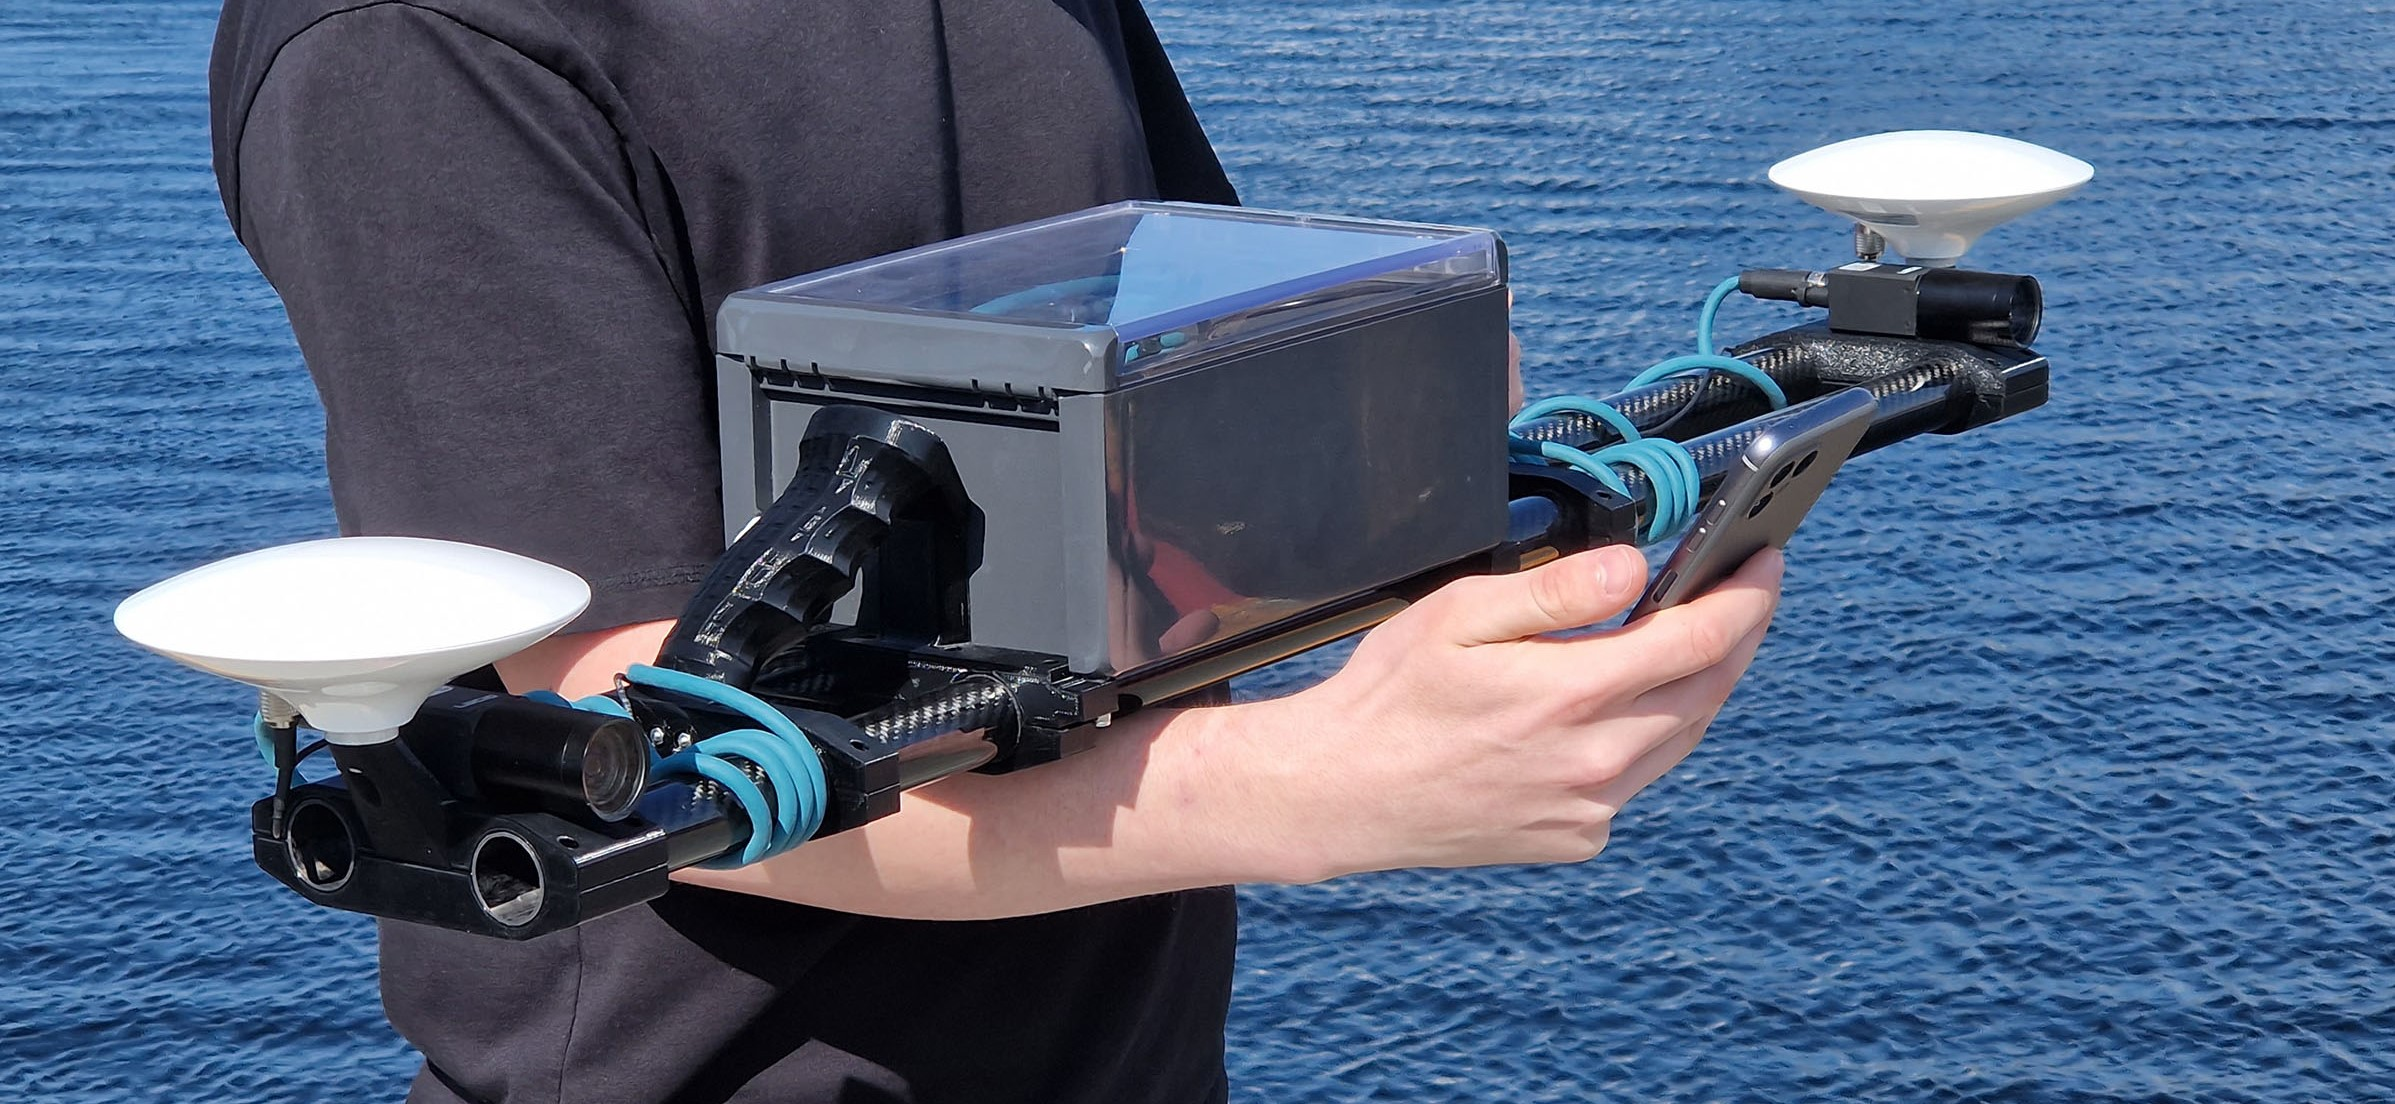
\includegraphics[width=0.9\textwidth]{figures/operation.jpg}
    \caption{Operation of the sensor rig.}
\end{figure}


\begin{figure}[H]
    % \centering
    \subcaptionbox{Scene as observed by a regular camera.}{
        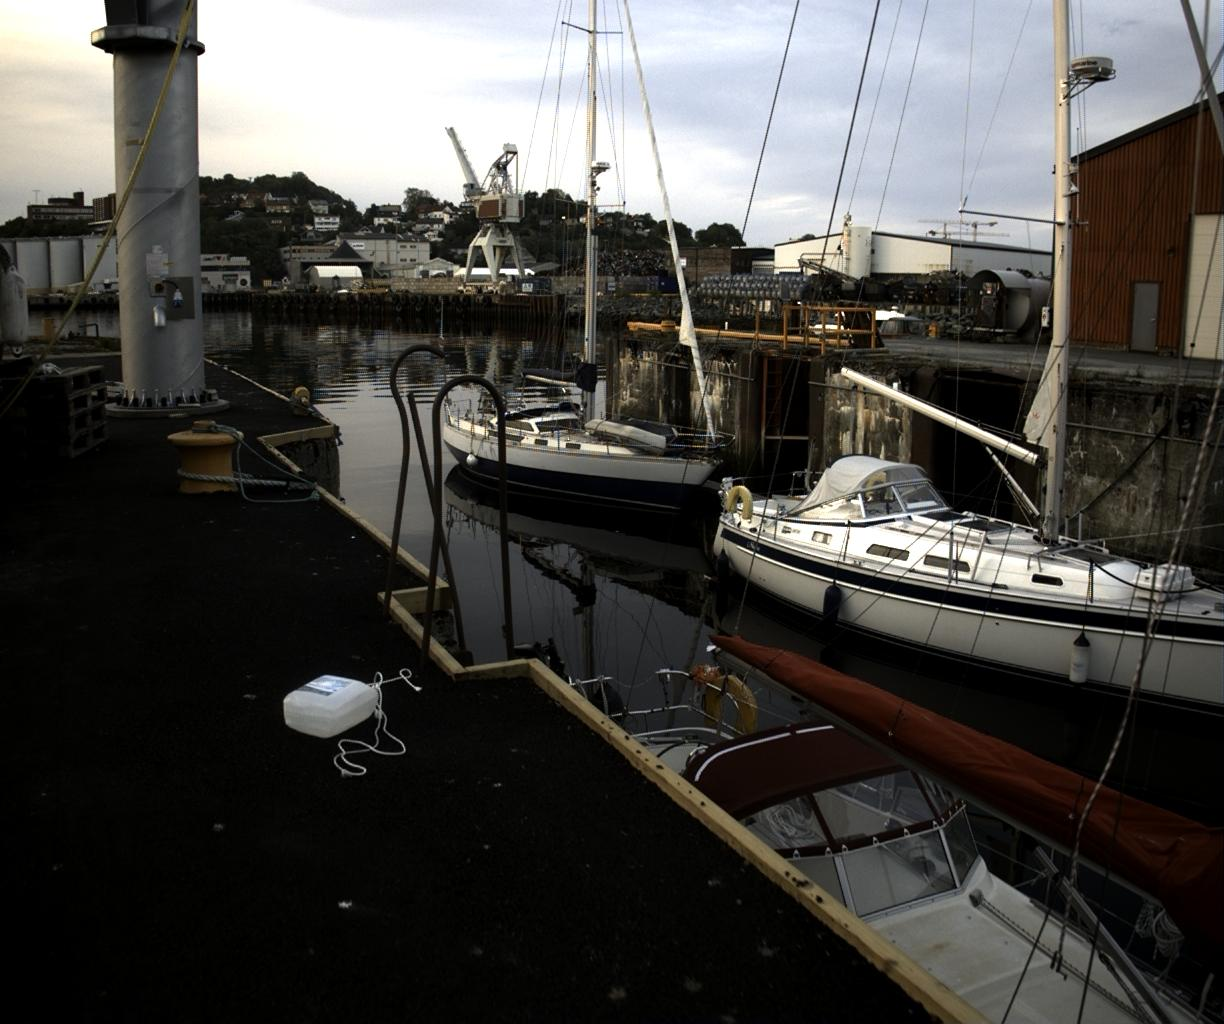
\includegraphics[width=0.48\textwidth]{figures/regular_right_96.jpeg}
    }
    \hfill
    \subcaptionbox{Visualization of raw polarization data with \glsentrylong{aolp} and \glsentrylong{dolp} visualized as hue and value of an HSV image.}{
        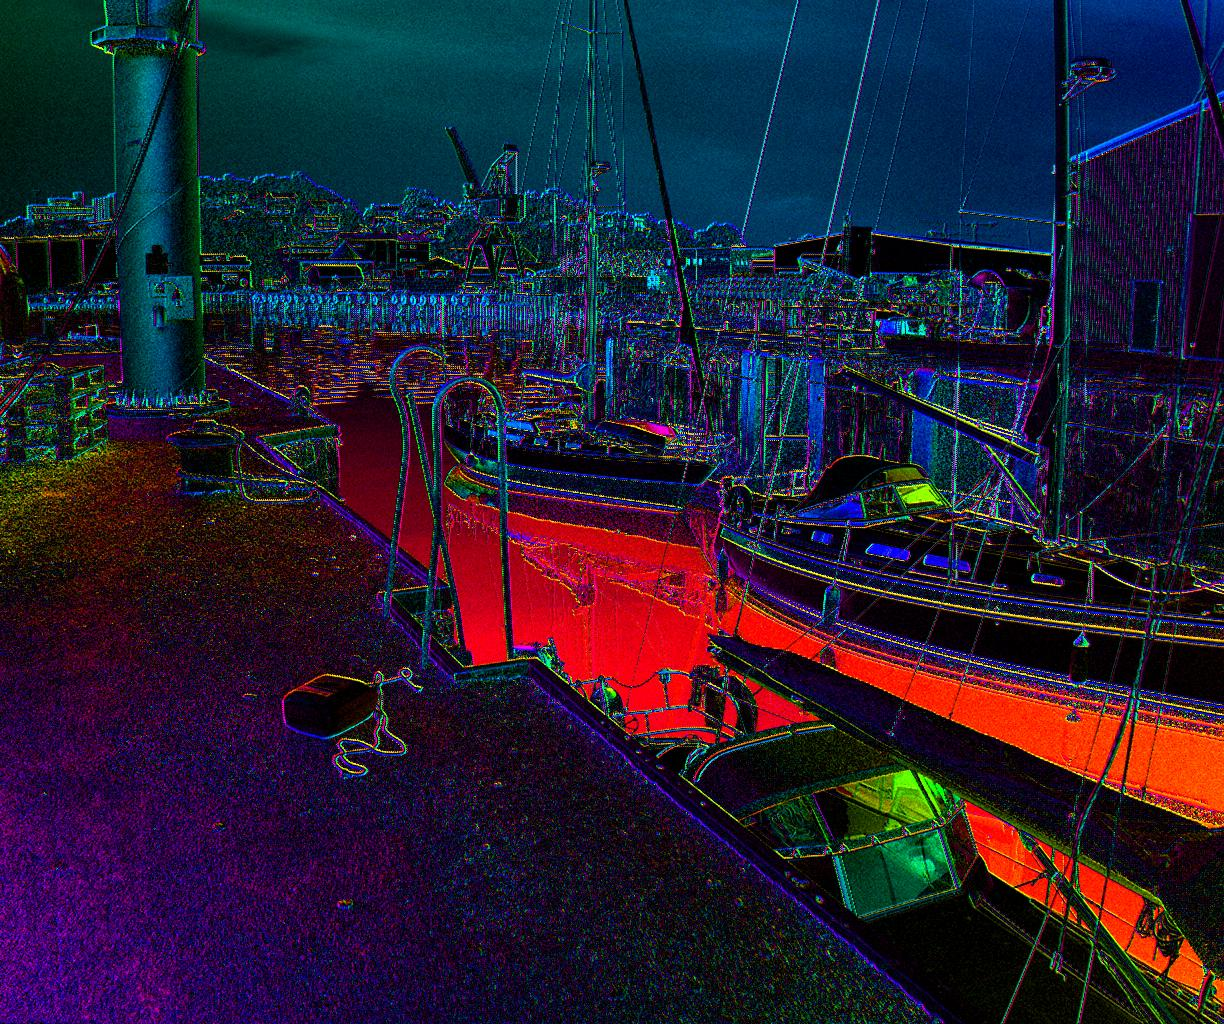
\includegraphics[width=0.48\textwidth]{figures/aolp_right_96.jpeg}
    }
    \caption{Illustration of how polarization cameras provide additional information in a maritime context.}
    \label{fig:polarization_visualization}
\end{figure}


\end{document}